%% RA-L: how a discovery candidate is formed, and why its geometry is not incidental.
%% This is the premise Table IV's columns rest on -- SAM's coverage is subtracted
%% BEFORE connected components are formed, so on an object the pipeline already had,
%% the only thing left to propose is the rim. Disjoint from the companion's
%% pipeline_end_to_end, which draws the per-mask agent execution order instead.
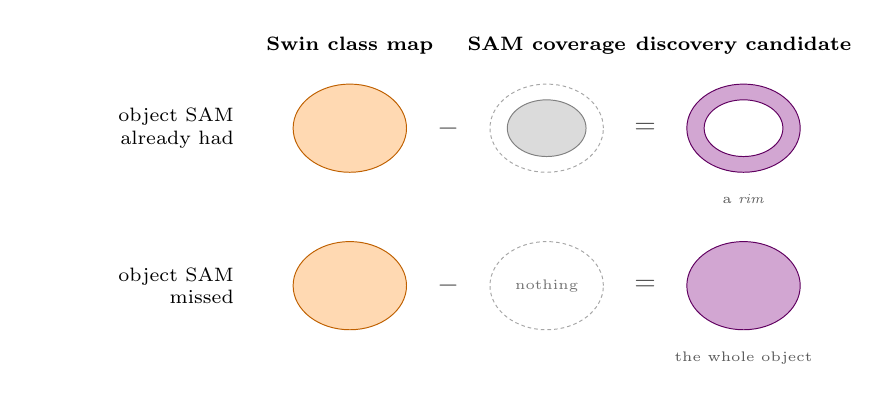
\begin{tikzpicture}[
  font=\scriptsize,
  swin/.style = {fill=orange!30, draw=orange!75!black, line width=0.35pt},
  sam/.style  = {fill=black!14,  draw=black!50,        line width=0.35pt},
  cand/.style = {fill=violet!35, draw=violet!75!black, line width=0.35pt},
  none/.style = {draw=black!35, dashed, dash pattern=on 1.3pt off 1.1pt, line width=0.35pt},
  colhdr/.style = {font=\scriptsize\bfseries, align=center},
  rowhdr/.style = {font=\scriptsize, align=right, text width=2.5cm},
  op/.style     = {font=\normalsize, text=black!70},
]

\def\ca{0}      % column x: Swin class map
\def\cb{2.5}    % column x: SAM coverage
\def\cc{5.0}    % column x: candidate
\def\ra{0}      % row y: object SAM already had
\def\rb{-2.0}   % row y: object SAM missed

% ---- column headers --------------------------------------------------------
\node[colhdr] at (\ca, 1.05) {Swin class map};
\node[colhdr] at (\cb, 1.05) {SAM coverage};
\node[colhdr] at (\cc, 1.05) {discovery candidate};

% ---- operators -------------------------------------------------------------
\node[op] at ({(\ca+\cb)/2}, \ra) {$-$};
\node[op] at ({(\cb+\cc)/2}, \ra) {$=$};
\node[op] at ({(\ca+\cb)/2}, \rb) {$-$};
\node[op] at ({(\cb+\cc)/2}, \rb) {$=$};

% ---- row A: an object SAM had already segmented ----------------------------
\node[rowhdr, anchor=east] at (-1.35, \ra) {object SAM\\already had};

\fill[swin] (\ca, \ra) ellipse (0.72 and 0.56);
\fill[sam]  (\cb, \ra) ellipse (0.50 and 0.36);
\draw[none] (\cb, \ra) ellipse (0.72 and 0.56);
\fill[cand, even odd rule] (\cc, \ra) ellipse (0.72 and 0.56)
                           (\cc, \ra) ellipse (0.50 and 0.36);
\node[font=\tiny, text=black!65, anchor=north] at (\cc, {\ra-0.72}) {a \emph{rim}};

% ---- row B: an object SAM missed entirely ----------------------------------
\node[rowhdr, anchor=east] at (-1.35, \rb) {object SAM\\missed};

\fill[swin] (\ca, \rb) ellipse (0.72 and 0.56);
\draw[none] (\cb, \rb) ellipse (0.72 and 0.56);
\node[font=\tiny, text=black!55] at (\cb, \rb) {nothing};
\fill[cand] (\cc, \rb) ellipse (0.72 and 0.56);
\node[font=\tiny, text=black!65, anchor=north] at (\cc, {\rb-0.72}) {the whole object};

\end{tikzpicture}
